\section{Analysis}

\subsection{Use Case analysis}

\subsubsection{Class Candidates}

\subsubsection{Description of Classes}

\subsubsection{UML Analysis Diagram}

\subsection{Use Case Realisation}

\subsubsection{Sequence Diagrams}

\subsubsection{Operation Contracts}

\subsubsection{Updated UML Class Diagram}
\begin{figure}[ht]
\centering 
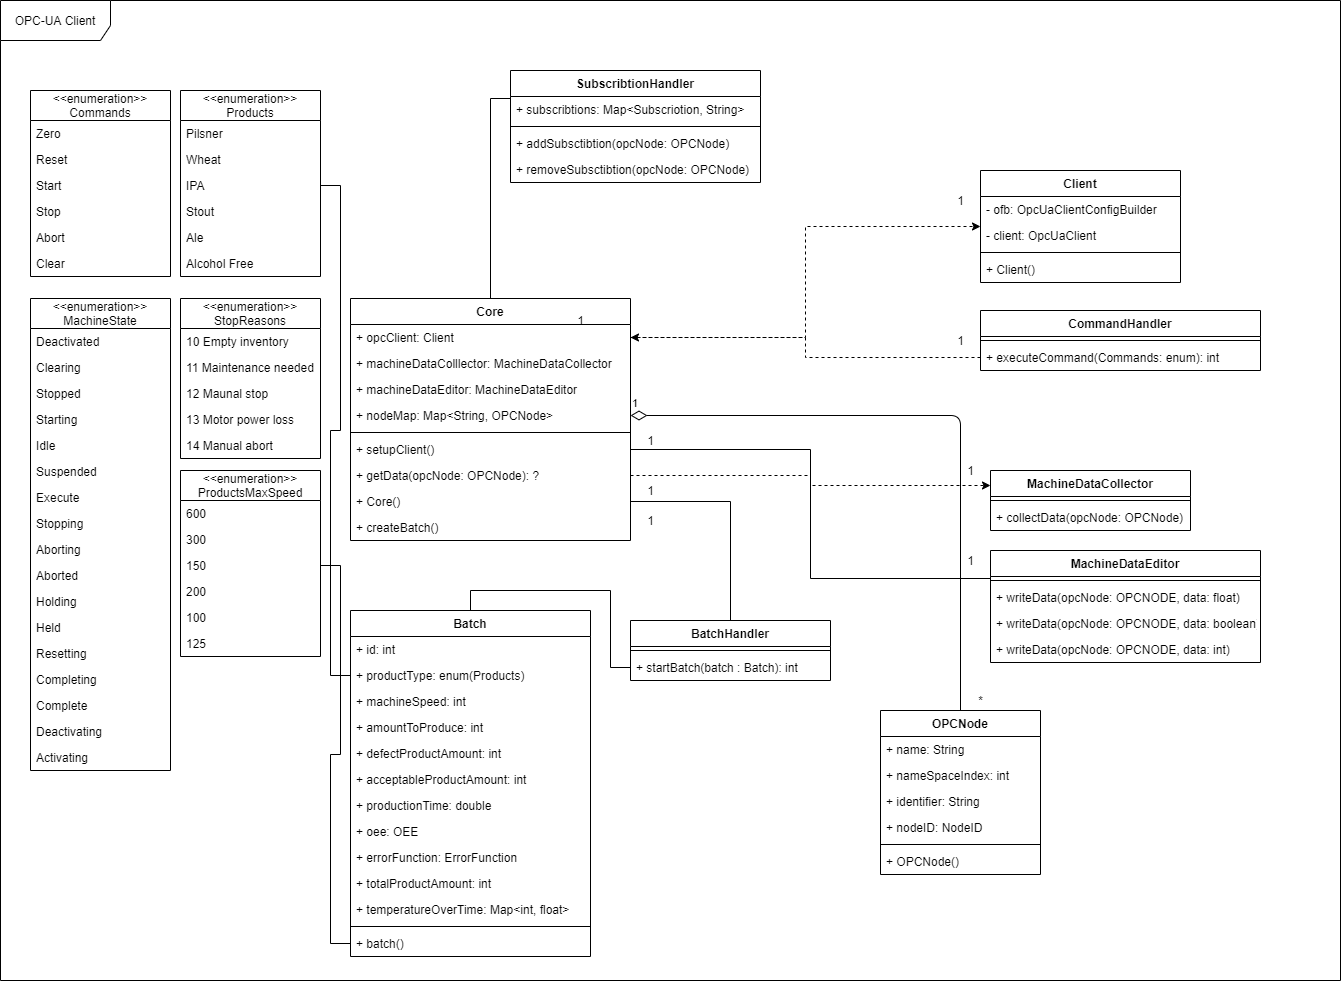
\includegraphics[scale=0.3]{images/diagrams/updated_UML_Class_Diagram.drawio.png}
\caption{Updated UML Class Diagram}
\label{figure:updated_UML_class_diagram} 
\end{figure}


The updated UML class diagram illustrates the current system idea based on the 
analysis of the system. Although this diagram only shows the 
OPC-UA client, it still gives a good idea of how this part of the system is going
to be, once implemented. \\

By using the diagram in the implementation phase, the group has a good starting 
point to expand on. The classes in the UML class diagram have a chance of not 
being implemented if the group finds them unuseful or changed to adhere to the 
program.